\documentclass[11pt,reqno]{amsart}
\usepackage[T1]{fontenc}\usepackage[utf8]{inputenc}\usepackage{lmodern}
\usepackage[a4paper,margin=25mm]{geometry}
\usepackage{amsmath,amssymb,mathtools,microtype,booktabs,graphicx,tikz}
\usepackage[hidelinks]{hyperref}
\newtheorem{theorem}{Theorem}\newtheorem{lemma}{Lemma}
\title{A global sign for the literal Erd\H{o}s--Straus receiving determinant}
\author{The Clankers}\date{21 September 2026}
\begin{document}
\begin{abstract}
An explicit quartic receiving matrix used in a recent ES/Split-Zero construction
has an additional determinantal divisor, distinct from its root discriminant.
We prove that divisor is avoided by every positive integral ES witness at every
prime $p\equiv1\pmod{12}$. Two exact polynomial certificates give uniform
negative bounds and an original-coordinate inverse bound. Real and $p$-adic
zeros do not contradict the result. No ES existence theorem is asserted.
\end{abstract}\maketitle

For positive integers $x,y,z$ with $4/p=1/x+1/y+1/z$, retain
$\ell=(p,x,y,z)$, $S=\sum\ell_i$, and the literal normalization
\[
 H(T)=-S^{-1}\prod_i(T-\ell_i)=AT^4+T^3+BT^2+CT+D.
\]
At simple roots choose and retain $\xi_i\in\mathbb C^\times$ with
$\xi_i^2H'(\ell_i)=1$. The sign-odd receiving matrix
$O\in M_4(\mathbb C)$ in the supplied programme has columns
\[
 o_i=\xi_i\bigl(1,-id_i,Ad_i^2+2\ell_id_i,
                         i(7\ell_i^2d_i-13d_i^2)\bigr)^T,
 \qquad d_i=H'(\ell_i).
\]
Put $V=\prod_{i<j}(\ell_j-\ell_i)$ and
$\epsilon=A^2V\prod_i\xi_i\in\{1,-1\}$. This retains root order and every
square-root choice. The determinant is
$\det O=4\epsilon F/A^3=-4\epsilon\mathfrak N/S^3$, where
\begin{align*}
 F={}&20(3C-B^2)+A(87B^3-282BC-51D)\\
 &+A^2(-28B^4+22B^2C+431C^2+204BD)\\
 &+A^3(224B^2D-168BC^2-856CD)-448A^4D^2.
\end{align*}
Reduction of the four component polynomials modulo $H$ proves this identity;
the supplied standard-library verifier checks it universally. Set
$\mathfrak N(\ell)=S^6F$. This is an integer homogeneous polynomial of degree
eight in integral $\ell$, without any assumption that $S$ is a $p$-unit.

\begin{theorem}
For every prime $p\equiv1\pmod{12}$ and every positive integral ES witness,
\[
 \boxed{\mathfrak N<-\frac{125873811}{262144}p^8<0.}
\]
For $p\equiv1\pmod{24}$ the stronger constant is
$c=327448292668/47045881$. With either applicable constant,
\[
 \boxed{|\det O|>\frac{4cp^8}{S^3},\qquad
             \|O^{-1}\|_2<\frac{360S^9}{cp^8}.}
\]
Here $\|\cdot\|_2$ is the operator norm for the standard Hermitian norm on
$\mathbb C^4$.
\end{theorem}

\paragraph{The complete original arithmetic domain.}
Four literal roots are distinct: $x=p$ would give
$(3y-p)(3z-p)=p^2$ with incompatible residues modulo three; $x=y=a$ gives
$4(2a-p)z=p(2a)$ and $2a-p\mid p^2$, whose three cases all fail integrality
for $p\equiv1\pmod4$. At least one, but not all, denominators are divisible
by $p$.

If two are, the third is the unique smallest denominator $a<p/2$. If only one
is $pk$, let the other two be $a\le b$, both units at $p$. Write
$4k-1=pt$, $a=gr$, $b=gs$, $(r,s)=1$. Then $k=drs$, $r+s=t\lambda$,
$g=d\lambda$, and $t\equiv3\pmod4$. The contrary inequality $a\ge p/2$
gives $2dr(r-s)\ge-1$, hence $r=s=1$ and $t\mid2$, impossible.
Thus every witness has $p/4<a<p/2$.

Put $R=4a-p$. The identity $(Ry-pa)(Rz-pa)=p^2a^2$ recovers the full original
Type I/II source \cite[\S2]{ET}, with $u\mid a^2$:
\[
\begin{array}{c|c|c}
&\text{gate}&\text{ordered denominator return}\\ \hline
E&R\mid4u+1&(a,(pa+a^2/u)/R,(pa+p^2u)/R)\\
M&R\mid a+u&(a,p(a+a^2/u)/R,p(a+u)/R).
\end{array}
\]
The original normalization is $(h,r,s)=(g^2/u,u/g,a/g)$, $g=(a,u)$.
The ordered divisor inverses are $a^2/(Ry-pa)$ and $pa^2/(Ry-pa)$.
Complementation exchanges only the two M tails and is retained.

An E state has $u\ge2$: $u=1$ would require $R\mid5$. Write $(\cdot/R)$ for
the Jacobi symbol and $(\cdot/p)$ for the Legendre symbol. Reciprocity
primewise on $a$ gives $(u/R)=(u/p)$, so its target $-1/4$ makes $(u/p)=-1$. When
$p\equiv1\pmod{24}$, two and three are residues, and therefore $u\ge5$.
For M, write the two tails as $pb<pc$. Since neither denominator is $p$,
$b\ge2$ and $c-b\ge1$ are original integer inequalities.

\paragraph{Exterior coefficient identity.}
Use real $u\ge1$ and $w=p/R>1$. The four normalized roots are
\[
 \left(1,\frac{w+1}{4w},\frac{w+1}{4}+\frac{(w+1)^2}{16wu},
                  \frac{w+1}{4}+wu\right).
\]
Define $P_E\in\mathbb Z[u,w]$ by the exact division
\begin{align*}
 -64u^2P_E(u,w)=\mathfrak N\bigl(&16wu,4u(w+1),\\
 &(w+1)(4wu+w+1),4wu(w+1+4wu)\bigr).
\end{align*}
It has bidegree $(12,16)$. Each of the following has 221 positive integer
coefficients, occupying the full $13\times17$ rectangle:
\[
 P_E(1+X,1+Y),\quad
 (uP_{E,u}-6P_E)(1+X,1+Y),\quad
 (wP_{E,w}-8P_E)(1+X,1+Y).
\]
The arrays are the finite certificate. Hence
\[
 Q_E(u,w)=\frac{P_E(u,w)}{2^{26}u^6w^8}
       =-\frac{\mathfrak N}{p^8}
\]
is strictly increasing in both arguments. Exact boundary evaluation gives
\[
 Q_E(2,1)=\frac{125873811}{262144},\qquad
 Q_E(5,1)=\frac{1310003654463}{12800000}
             >\frac{327448292668}{47045881}.
\]
This proves both required bounds in the exterior channel.

\paragraph{Middle coefficient identity.}
Let $L=4bc-b-c$, $T=(b+c)L+bc$, $V=b^2c^2$. Then $a/p=bc/L$ and
$-\mathfrak N/p^8=\mathcal P(T/L,V/L)$, where
\begin{align*}
\mathcal P(s,v)={}&7168v^4-(5568s^2+5728s-5888)v^3\\
&+(320s^4+2744s^3+705s^2-3350s-903)v^2\\
&+(-140s^5-443s^4+440s^3+390s^2+70s-249)v\\
&+20s^6-7s^5-26s^4-7s^3+20s^2.
\end{align*}
Put
\[
 H_M(X,Y)=\left[L^6\mathcal P(T/L,V/L)\right]_{b=2+X,\,c=3+X+Y},
\]
\[
 L_M=4X^2+4XY+18X+7Y+19.
\]
The polynomial $47045881H_M-327448292668L_M^6$ has zero constant and 191
positive nonzero integer coefficients. Its $X$ and $Y$ coefficients are
positive. Dividing by $47045881L_M^6$ proves the stronger bound for all
$X,Y\ge0$. Equality requires $b=2,c=3$, hence $a=6p/19$, which is not integral
at a prime $p\equiv1\pmod{12}$. The inequality in the theorem is strict.

\begin{figure}[ht]
\centering
\resizebox{\textwidth}{!}{%
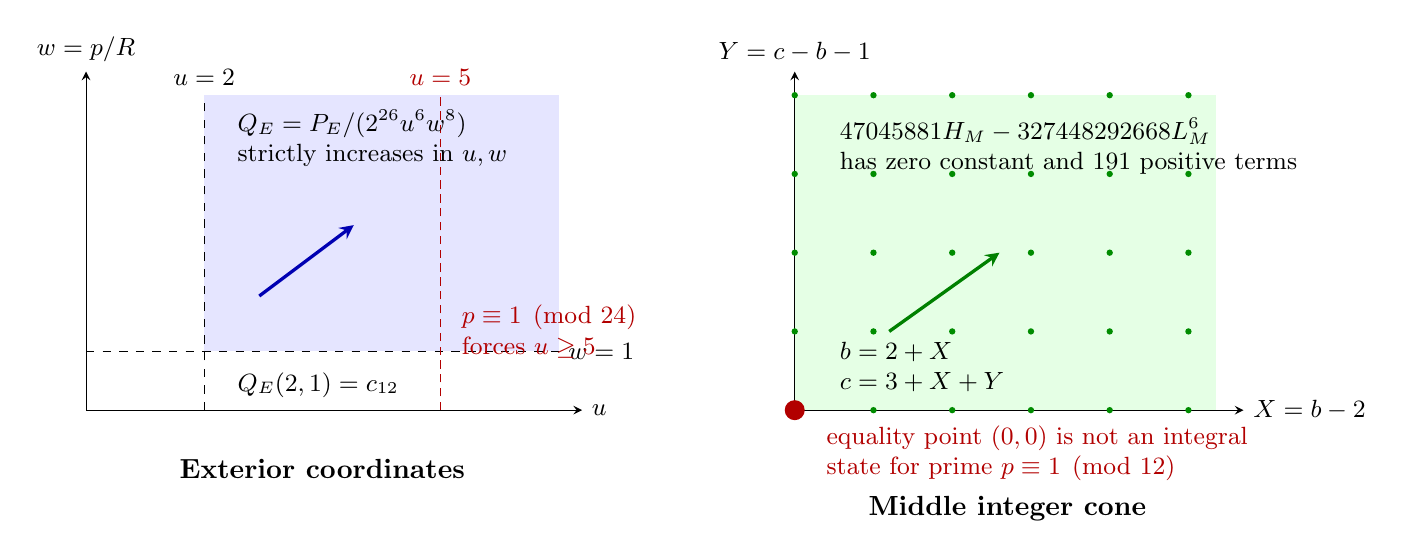
\begin{tikzpicture}[font=\small,>=stealth]
  % Exterior cone.
  \begin{scope}[xshift=0cm]
    \draw[->] (0,0) -- (6.3,0) node[right] {$u$};
    \draw[->] (0,0) -- (0,4.3) node[above] {$w=p/R$};
    \fill[blue!10] (1.5,0.75) rectangle (6,4);
    \draw[dashed] (0,0.75) -- (6,0.75) node[right] {$w=1$};
    \draw[dashed] (1.5,0) -- (1.5,4) node[above] {$u=2$};
    \draw[densely dashed,red!70!black] (4.5,0) -- (4.5,4) node[above] {$u=5$};
    \draw[->,very thick,blue!70!black] (2.2,1.45) -- (3.4,2.35);
    \node[align=left,anchor=west] at (1.8,3.45)
      {$Q_E=P_E/(2^{26}u^6w^8)$\\strictly increases in $u,w$};
    \node[align=left,anchor=west] at (1.8,0.32)
      {$Q_E(2,1)=c_{12}$};
    \node[align=left,anchor=west,red!70!black] at (4.65,1.0)
      {$p\equiv1\pmod{24}$\\forces $u\ge5$};
    \node[font=\bfseries] at (3,-0.75) {Exterior coordinates};
  \end{scope}

  % Middle cone.
  \begin{scope}[xshift=9cm]
    \draw[->] (0,0) -- (5.7,0) node[right] {$X=b-2$};
    \draw[->] (0,0) -- (0,4.3) node[above] {$Y=c-b-1$};
    \fill[green!10] (0,0) rectangle (5.35,4);
    \foreach \x in {0,...,5}{\foreach \y in {0,...,4}{\fill[green!55!black] (\x,\y) circle (1.15pt);}}
    \draw[->,very thick,green!50!black] (1.2,1.0) -- (2.6,2.0);
    \draw[fill=white,very thick,red!70!black] (0,0) circle (3pt);
    \node[align=left,anchor=west] at (0.45,3.35)
      {$47045881H_M-327448292668L_M^6$\\has zero constant and $191$ positive terms};
    \node[align=left,anchor=west] at (0.45,0.55)
      {$b=2+X$\\$c=3+X+Y$};
    \node[align=left,anchor=west,red!70!black] at (0.28,-0.55)
      {equality point $(0,0)$ is not an integral\\state for prime $p\equiv1\pmod{12}$};
    \node[font=\bfseries] at (2.7,-1.25) {Middle integer cone};
  \end{scope}
\end{tikzpicture}
}%
\caption{The two exact coordinate domains used in the global sign proof.  The
blue and green regions are certificate domains; actual Erd\H{o}s--Straus
witnesses are the arithmetic points satisfying the displayed gates and
integrality conditions.  The exterior lower bound is approached at the dashed
boundary $w=1$, which is excluded by $R<p$.  The middle comparison is strict at
every admissible lattice point because its only equality point would require
$a=6p/19$.}
\label{fig:coordinate-domains}
\end{figure}


\paragraph{Why the finite certificate is a proof.}
The source norm is the literal $F$ of \cite[Track I, E1]{Frame}, not a fitted array.
The main program expands every rational coefficient identity exactly, then
checks all its coefficients. The separate implementation proves the exterior
identity on the entire $17\times17$ unisolvent grid after clearing its known
bidegree $(16,16)$ denominator. It independently performs the two derivative
and binomial-translation operations. For M, it checks
\[
 \mathfrak N(L,bc,bL,cL)=-L^2H_M
\]
on the full $25\times17$ grid in $X,Y$, covering bidegree $(24,16)$, then
independently expands the comparison with $L_M^6$. Repeated one-variable
polynomial uniqueness makes these universal identities. This is a
computer-assisted coefficient lemma, not a finite-prime extrapolation.

\paragraph{Original inverse and norm.}
Let $\mathsf C_H$ be the reduction matrix of the four original component
polynomials, including their $i$ factors, and $U_{nj}=\ell_j^n\xi_j$.
Then $O=\mathsf C_HU$. Given $z$, set $m=\mathsf C_H^{-1}z$ using its adjugate.
Lagrange interpolation returns
\begin{align*}
 \beta_j=\xi_j\bigl[&(C+B\ell_j+\ell_j^2+A\ell_j^3)m_0
 +(B+\ell_j+A\ell_j^2)m_1\\
 &+(1+A\ell_j)m_2+A m_3\bigr].
\end{align*}
For four distinct integer roots, $2/S\le|d_j|\le S^2$. The entry bounds by row are
$\sqrt{S/2}$, $S$, $3S^2$ and $20S^3$. Every cofactor is at most $360S^6$;
the adjugate Frobenius norm is at most $1440S^6$. Dividing by
$4cp^8/S^3$ proves the inverse bound. Original positive metrics $G,Q$
contribute the explicit factor $\|G^{1/2}\|\,\|Q^{-1/2}\|$.

\paragraph{Scope and negative controls.}
At $p=1009$, the genuine E and M returns from $(a,u)=(253,11)$ are
$(253,87032,3818056)$ and $(253,2042216,88792)$. They violate two of the audit's
three sufficient character conditions, but are covered here. This does not
assert $p\nmid\mathfrak N$: their valuations are zero and two.

At $p=1$, let $b=t$, $c=t+1/10$, $a=bc/(4bc-b-c)$ for $3\le t\le4$.
The literal roots stay positive and distinct. Exact elimination produces a
degree-$18$ numerator $P(t)$ with all coefficients of $P'(3+X)$ positive and
opposite signs at $3053/1000$ and $1527/500$. Hence this real family has one
receiver singularity, at $t\approx3.05367681075890$. Its tail gap is not the
original integer gap used above. The earlier local zeros likewise remain local,
not integral, counterdomains.

Finally $p=1009,a=321,u=9$ gives the unfiltered E triple
$(321,335338/275,9486618/275)$. Its frame is nonsingular, but its E gate is
not satisfied: $275\nmid37$. Its $S^6F$ is rational, not an integer numerator.
Thus the theorem excludes receiver singularity conditional on an existing
positive integral witness at $p\equiv1\pmod{12}$; it does not establish
universal occupancy of the ES source. No priority determination, independent
human review, or Lean build is claimed.

\begin{thebibliography}{4}
\bibitem{ET} Elsholtz, C., \& Tao, T. (2013). Counting the number of solutions
to the Erd\H{o}s--Straus equation on unit fractions.
\emph{Journal of the Australian Mathematical Society, 94}(1), 50--105.
\href{https://arxiv.org/abs/1107.1010}{arXiv:1107.1010v6}.
Type I/II antecedents: source \S2, Propositions 2.2 and 2.6.
\bibitem{Receiver} The Clankers. (2026, September 20).
\emph{The odd receiving divisor pulled back to the Erd\H{o}s--Straus locus}.
\href{https://github.com/KokunoYumeto/erdos-straus-foundation/blob/49976b17491ba927df8bc7f2c2f81d39dfb15ce8/research/incoming/es-fable-zeta-bridge-20260920/ODD_RECEIVER_ES_PULLBACK.tex\#L19-L215}{Pinned source, EZ37--EZ48}.
\bibitem{Frame} The Clankers. (2026, September 20).
\emph{ES--RH continuation B: Arithmetic nonsingularity, paired determinant
bounds, finite heat actions, and arithmetic descent}. Erd\H{o}s--Straus Foundation,
\href{https://github.com/KokunoYumeto/erdos-straus-foundation/blob/49976b17491ba927df8bc7f2c2f81d39dfb15ce8/research/incoming/es-rh-continuation-b-20260920/RESEARCH_CONTINUATION.md\#L44-L254}{revision \texttt{49976b1}, Track I, E1--E6}.
The polynomial and three-character theorem were read directly at this revision.
\bibitem{Descent} The Clankers. (2026, September 21).
\emph{Original-divisor descent from rational Erd\H{o}s--Straus trace sources}.
\href{https://github.com/KokunoYumeto/erdos-straus-foundation/blob/1400e6301429cf9c66d8071e107be9dc41f5b907/research/incoming/es-turn07-divisor-descent-20260921/core.tex\#L1-L16}{Pinned scope and initial-occupancy boundary}.
\end{thebibliography}
\end{document}
